\documentclass[manuscript,review,anonymous]{acmart}

\usepackage{booktabs}
\usepackage{graphicx}
\usepackage{amsmath}
\usepackage{listings}
\usepackage{xcolor}
\usepackage{enumitem}

\lstset{
  basicstyle=\ttfamily\small,
  backgroundcolor=\color{gray!10},
  frame=single,
  breaklines=true,
  keywordstyle=\color{blue},
  commentstyle=\color{green!50!black},
  stringstyle=\color{red!60!black},
}

\copyrightyear{2026}
\acmYear{2026}

\begin{document}

\title{Neuriphonium: Real-Time Brainwave-to-Music Mapping for Improvisational Performance}

\author{ANONYMOUS AUTHOR(S)}
\affiliation{%
  \institution{Anonymous Institution}
  \city{Anonymous City}
  \country{Anonymous Country}
}

\begin{abstract}
We present Neuriphonium, a real-time system that captures the ``vibe'' of a performer's brainwave activity and translates it into continuously evolving musical textures suitable for live improvisation with an acoustic instrument. Unlike prior brain-computer musical interfaces (BCMIs) that rely on discrete emotional state classification or threshold-based parameter switching, Neuriphonium employs a continuous, proportional mapping from EEG frequency bands to generative music parameters---including sampling temperature, top-$k$ filtering, classifier-free guidance strength, drum conditioning, and style embeddings. The system streams raw EEG data from a consumer-grade Muse headband (4-channel, TP9/AF7/AF8/TP10), computes five-band power ratios (delta, theta, alpha, beta, gamma) via FFT, derives higher-level affective metrics (arousal, valence, focus, relaxation), and feeds these into Magenta RealTime 2, a streaming neural audio generation model running locally on Apple Silicon via MLX. A layered vibe prompt builder constructs natural-language style descriptions from band proportions, which are embedded and smoothly interpolated to avoid abrupt musical discontinuities. We additionally contribute an EEG fingerprinting pipeline using LaBraM pretrained transformer embeddings to verify that distinct listening states (e.g., trash metal vs.\ Gregorian chant) produce separable neural signatures (97--100\% KNN accuracy), validating the premise that brainwave activity carries genre-discriminative information. The system operates with a real-time ratio of 2.5--3.0$\times$ on Apple M-series hardware, enabling uninterrupted audio streaming at 48\,kHz stereo.
\end{abstract}

\keywords{Brain-Computer Interface, EEG, Generative Music, Real-Time Audio, Magenta, Music Improvisation, Neurofeedback}

\ccsdesc[500]{Human-centered computing~{~}Interaction paradigms~{~}Interaction devices}
\ccsdesc[300]{Applied computing~{~}Sound and music computing}
\ccsdesc[300]{Computing methodologies~{~}Machine learning~{~}Neural networks}

\maketitle

\section{Introduction}

The intersection of brain-computer interfaces (BCIs) and music generation has historically been divided into two camps: systems that use EEG as a control signal for pre-composed musical parameters (tempo, pitch, volume), and systems that generate music from scratch based on classified emotional states. Both approaches share a common limitation: they treat the brain as a discrete controller, mapping threshold-crossing events to musical changes. This produces abrupt transitions that are musically jarring and unsuitable for the fluid, continuous nature of improvisational performance.

Neuriphonium addresses this gap by treating the brain as a \emph{continuous vibe source}---a multi-dimensional signal whose five frequency bands (delta, theta, alpha, beta, gamma) each contribute proportionally to the evolving musical texture. Rather than asking ``is the user relaxed or focused?'' and switching between predefined musical styles, the system asks ``what is the \emph{blend} of neural activity right now?'' and modulates generative parameters accordingly.

The system is designed for a specific use case: a musician wearing a Muse EEG headband while playing an acoustic instrument, with the generated music serving as a responsive, evolving accompaniment that mirrors the performer's mental state in real time. The generated audio must therefore be (1) continuous and uninterrupted, (2) responsive to subtle brainwave changes without abrupt shifts, and (3) musically rich enough to support improvisation.

Our contributions are:
\begin{itemize}[nosep]
  \item A \textbf{continuous proportional mapping} from EEG band powers to generative music parameters (temperature, top-$k$, CFG guidance, drum conditioning), replacing discrete threshold-based approaches.
  \item A \textbf{layered vibe prompt builder} that constructs natural-language style descriptions from band proportions, enabling fine-grained control over musical texture, energy, mood, space, and instrumentation.
  \item A \textbf{smooth style embedding interpolation} mechanism that prevents abrupt musical discontinuities when the brain state shifts.
  \item A \textbf{thread-safe real-time architecture} that decouples EEG processing, style embedding computation, and audio generation to maintain uninterrupted playback.
  \item An \textbf{EEG fingerprinting pipeline} using LaBraM pretrained embeddings to verify that different listening states produce separable neural signatures.
\end{itemize}

\section{Related Work}

\subsection{Brain-Computer Musical Interfaces}

The concept of Brain-Computer Musical Interfaces (BCMIs) was introduced by Miranda~\cite{miranda2010} as an extension of traditional BCIs that maps neural signals to musical processes rather than motor control. Early BCMIs used spectral features of EEG to trigger pre-composed musical events or control synthesizer parameters. BrainiBeats~\cite{brainibeats2023} extended this to dual-brain scenarios, using inter-brain synchrony to manipulate musical intervals. MindMusic~\cite{mindmusic2019} used a Muse headband with the Impro-Visor jazz improvisation system, mapping alpha waves to note durations. Reflex-in~\cite{reflexin2023} used Web Audio and WebSocket technologies for browser-based brainwave sonification.

A common limitation across these systems is their reliance on either (a) rule-based music generation with limited expressivity, or (b) discrete state classification that produces abrupt musical transitions. Neuriphonium advances the field by using a state-of-the-art streaming neural audio model (Magenta RealTime 2) with continuous parameter modulation.

\subsection{EEG-Based Emotion Recognition for Music}

Prior work has established that EEG frequency bands correlate with affective states: beta and gamma power correlate with arousal~\cite{russell1980}, frontal alpha asymmetry correlates with valence~\cite{davidson2004}, and the theta/beta ratio indexes attentional control~\cite{putman2014}. Systems such as Mind to Music~\cite{mindtomusic2024} use EEG emotion recognition to drive real-time music generation. A minimalist BCMI using two prefrontal electrodes~\cite{minimalistbcmi} demonstrated that even low-cost hardware can support affective sonification, though frontal alpha asymmetry alone did not reliably distinguish instructed emotional states. Tiraboschi et al.~\cite{tiraboschi2021} proposed a BCMI using MusicVAE conditioned on valence and arousal estimated from EEG, introducing a probabilistic mapping from affective dimensions to the model's latent space.

Neuriphonium uses a richer feature set---five-band power ratios plus four derived metrics---and maps them continuously rather than classifying them into discrete emotional categories.

\subsection{Generative Music Models}

Magenta RealTime 2 (mrt2\_small, 230M parameters)~\cite{livemusicmodels} is a streaming neural audio generation model that produces 48\,kHz stereo audio in 1-second chunks (25 frames). It is a codec language model built on three components: SpectroStream~\cite{spectrostream}, a neural audio codec that tokenizes 48\,kHz stereo audio; MusicCoCa~\cite{livemusicmodels}, a contrastive captioner that embeds text and audio into a shared 768-dimensional space (building on CoCa~\cite{coca} and MuLan~\cite{mulan}); and a decoder-only Transformer that generates audio tokens conditioned on style embeddings and optional MIDI control. The model maintains a streaming state across chunks, enabling continuous generation with a real-time factor of 1.6$\times$ on Colab TPUs. On Apple Silicon via MLX, the mrt2\_small variant achieves 2.5--3.0$\times$ real-time ratio. Google's Lyria RealTime API offers an alternative cloud-based generation path with extended controls.

\section{System Architecture}

Neuriphonium consists of four concurrent subsystems running in an asyncio event loop (Figure~\ref{fig:architecture}):

\begin{enumerate}[nosep]
  \item \textbf{EEG Acquisition}: Streams 4-channel EEG data from a Muse headband via Lab Streaming Layer (LSL), with automatic reconnection on stream loss.
  \item \textbf{Signal Processing}: Computes band powers, affective metrics, and musical parameters from sliding windows of EEG data.
  \item \textbf{Music Generation}: Runs Magenta RealTime 2 locally (or Lyria 3 online) to produce streaming audio conditioned on the current brain state.
  \item \textbf{Web Dashboard}: A WebSocket server that broadcasts EEG visualizations and audio chunks to a browser-based interface for real-time monitoring and control.
\end{enumerate}

\begin{figure}[h]
  \centering
  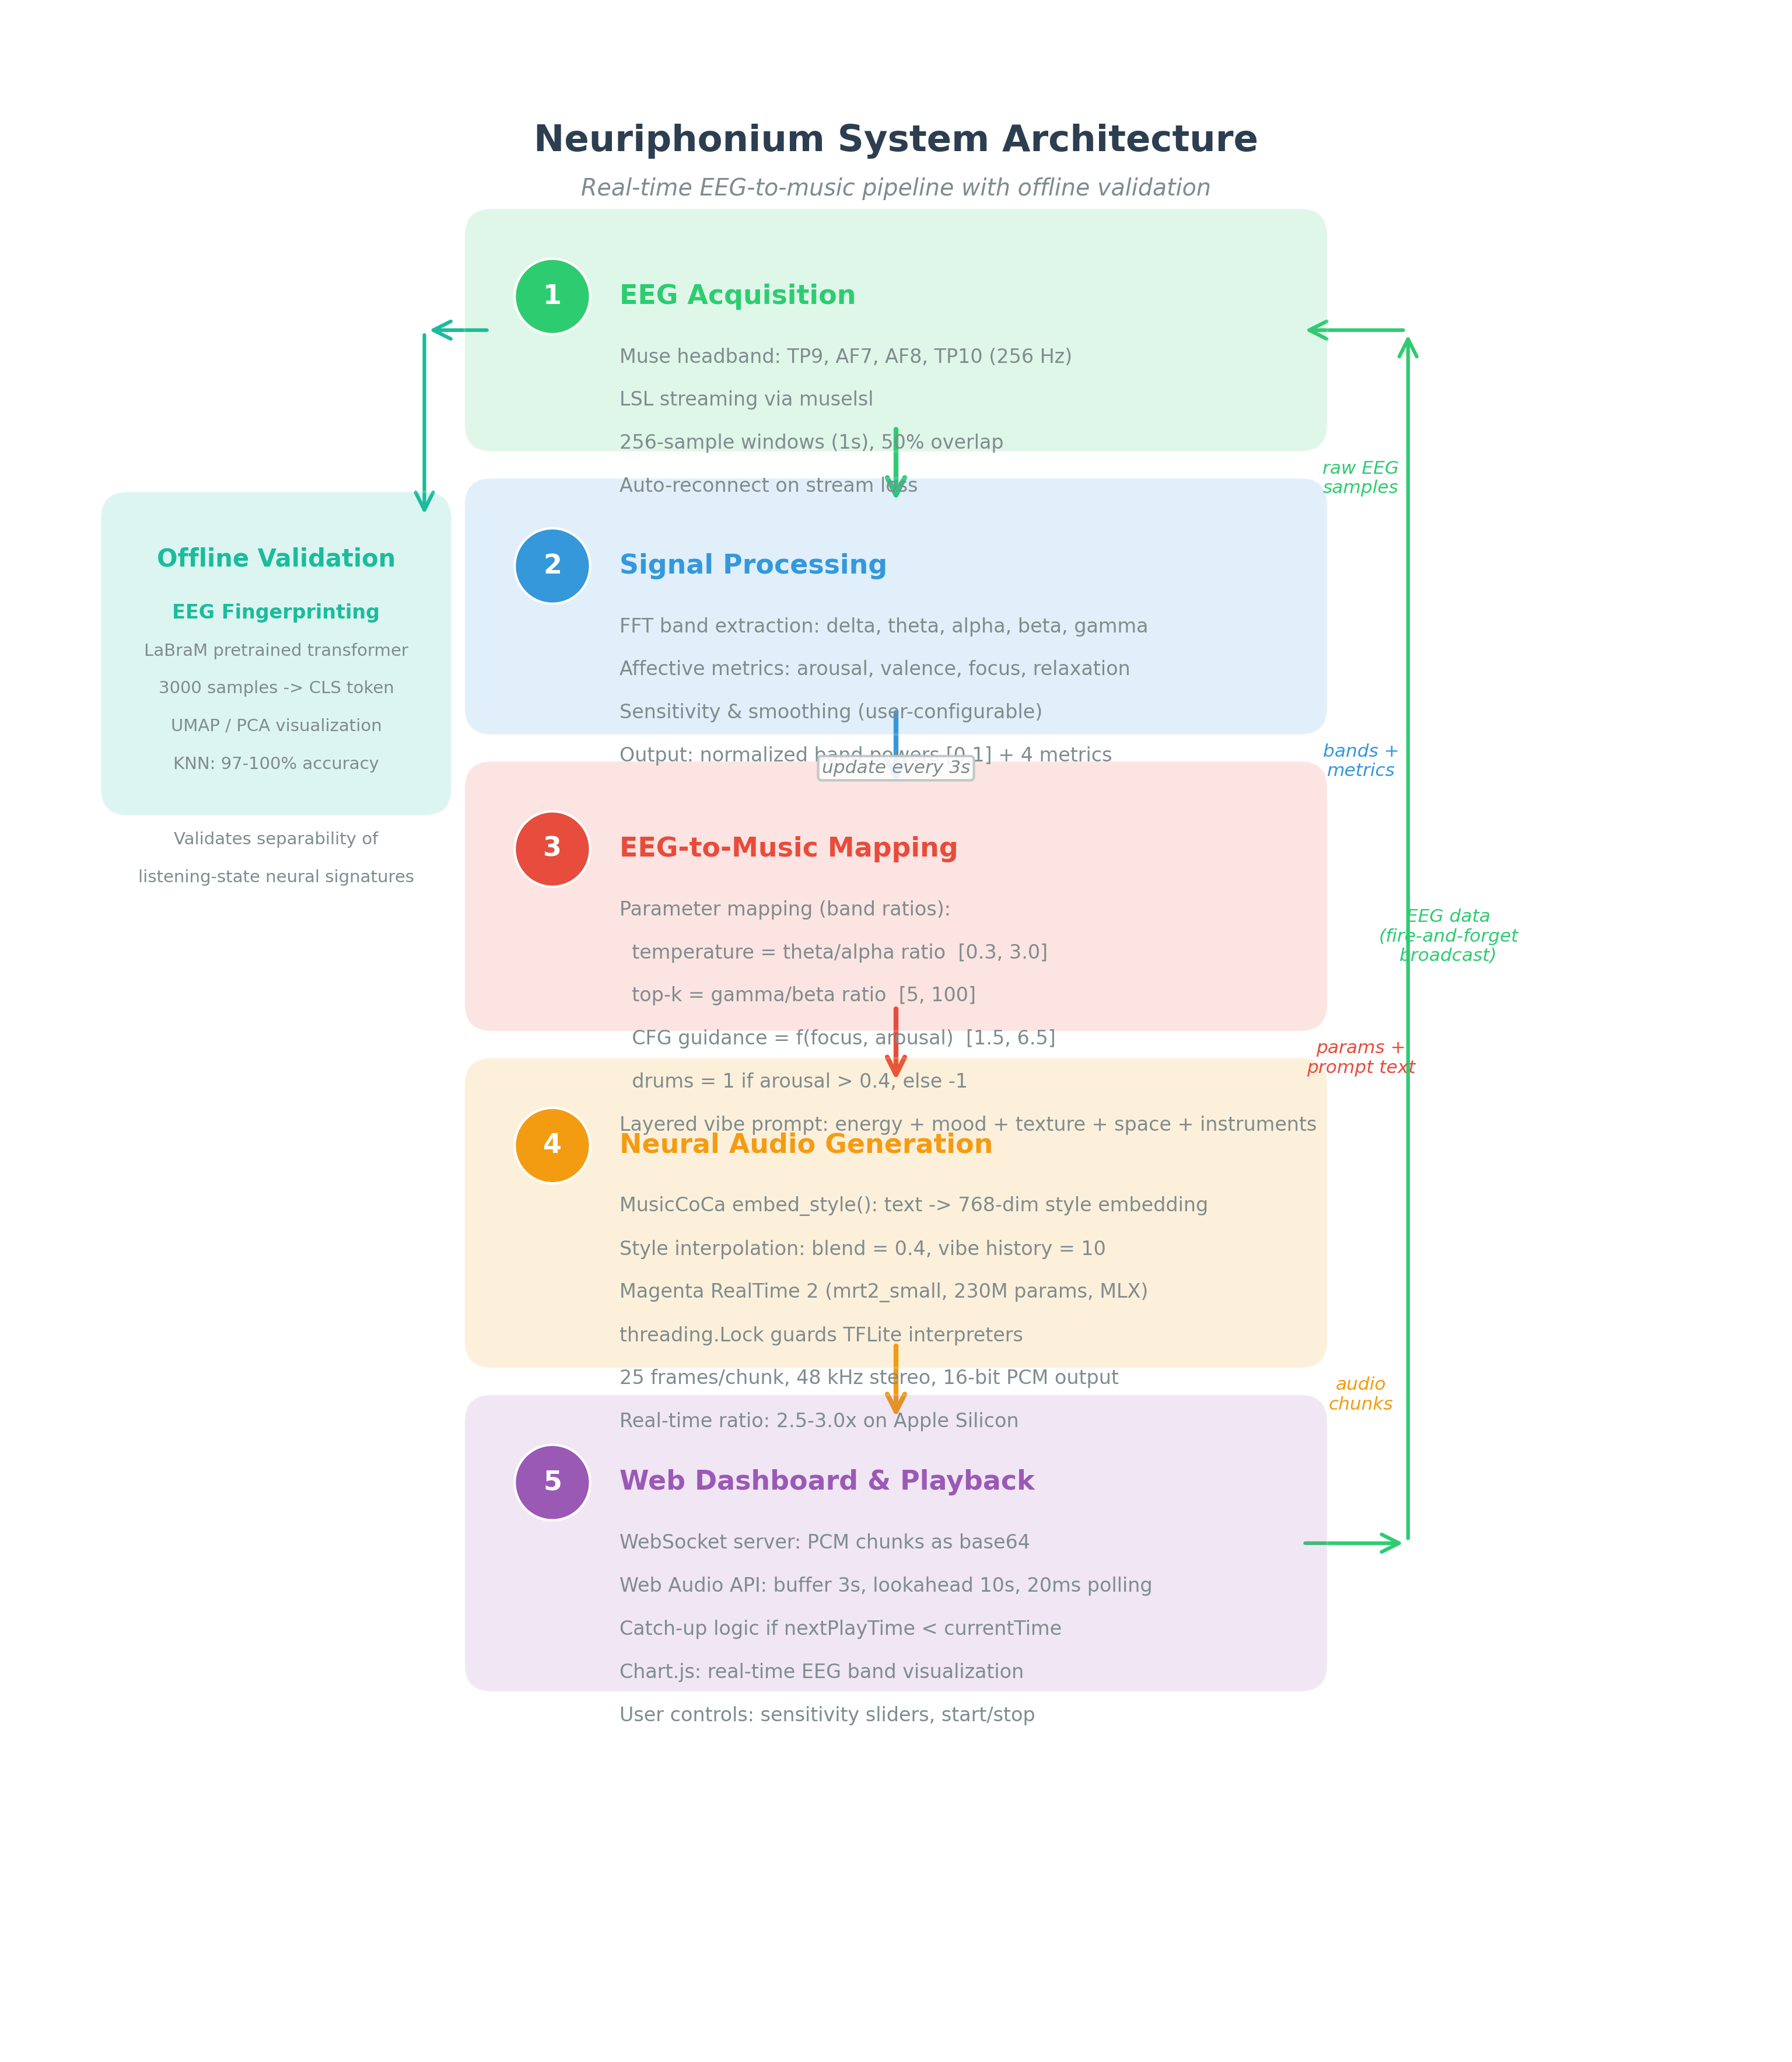
\includegraphics[width=\linewidth]{architecture.png}
  \caption{System architecture. Five-stage pipeline from EEG acquisition to web playback, with an offline validation branch using LaBraM embeddings.}
  \label{fig:architecture}
\end{figure}

\subsection{EEG Acquisition}

The system connects to a Muse headband via the Lab Streaming Layer (LSL) protocol. The Muse provides four EEG channels at positions TP9, AF7, AF8, and TP10, sampled at 256\,Hz when streamed via \texttt{muselsl}. A background reconnection task polls for LSL streams every 3 seconds if the connection is lost, ensuring robustness during live performance. When no stream is available, the system falls back to simulated sinusoidal data to maintain operation.

Samples are accumulated into a buffer of 256 samples (1 second at 256\,Hz), with a 50\% overlap between consecutive windows (\texttt{WINDOW\_SIZE // 2}).

\subsection{Signal Processing}

\subsubsection{Band Power Extraction}

For each 256-sample window, the system computes the Fast Fourier Transform (FFT) across all four channels and extracts average power in five frequency bands:

\begin{equation}
  \text{power}_{\text{band}} = \frac{1}{N_{\text{chan}}} \sum_{c=1}^{N_{\text{chan}}} \frac{1}{|F_{\text{band}}|} \sum_{f \in F_{\text{band}}} |X_c(f)|^2
\end{equation}

where $F_{\text{band}}$ is the set of frequency bins within the band's range (Table~\ref{tab:bands}). Powers are then normalized to relative proportions:

\begin{equation}
  p_{\text{band}} = \frac{\text{power}_{\text{band}}}{\sum_{b} \text{power}_b}
\end{equation}

Each band power is further adjusted by a per-band sensitivity multiplier (configurable from the UI, range 0--3$\times$) and smoothed using a rolling mean over a configurable window (default 3 samples).

\begin{table}[h]
  \caption{EEG frequency bands and their musical semantics.}
  \label{tab:bands}
  \begin{tabular}{lll}
    \toprule
    Band & Range (Hz) & Musical Mapping \\
    \midrule
    Delta ($\delta$) & 0.5--4 & Bass depth, gravity, predictability \\
    Theta ($\theta$) & 4--8 & Dreamy atmosphere, creative unpredictability \\
    Alpha ($\alpha$) & 8--13 & Smooth melodies, stability, consonance \\
    Beta ($\beta$) & 13--30 & Precise rhythms, structure, focus \\
    Gamma ($\gamma$) & 30--50 & Sparkling details, complexity, variety \\
    \bottomrule
  \end{tabular}
\end{table}

\subsubsection{Affective Metrics}

From the normalized band powers, the system derives four higher-level metrics:

\begin{align}
  \text{arousal} &= \text{clip}(0.1\delta + 0.2\theta + 0.3\alpha + 0.5\beta + 0.7\gamma, 0, 1) \\
  \text{valence} &= \text{clip}(\alpha - 0.3\theta - 0.2|\beta - \theta| + 0.5, 0, 1) \\
  \text{focus} &= \text{clip}\left(\frac{\beta}{3(\theta + 0.01)}, 0, 1\right) \\
  \text{relaxation} &= \text{clip}\left(\frac{\alpha}{2(\beta + 0.01)}, 0, 1\right)
\end{align}

These metrics are computed relative to a baseline established during the first 5 windows of data. A configurable global sensitivity parameter (default 2.5$\times$) amplifies deviations from baseline:

\begin{equation}
  \text{metric}_{\text{adjusted}} = \text{clip}(\text{baseline} + (\text{metric} - \text{baseline}) \times \text{sensitivity}, 0, 1)
\end{equation}

\subsection{Continuous Vibe-to-Music Mapping}

The core innovation of Neuriphonium is the replacement of discrete threshold-based mappings with continuous, proportional relationships between EEG bands and generative parameters.

\subsubsection{Parameter Mapping}

Four generative parameters are continuously modulated:

\paragraph{Temperature.}
Sampling temperature controls the randomness of token prediction. Rather than using absolute band values, we use the \emph{ratio} of theta to alpha, which amplifies small fluctuations in the creative/stable balance:

\begin{equation}
  T_{\text{target}} = \text{clip}\left(0.5 + \frac{\theta}{\alpha + 0.01} \times 1.2 + 0.8 \times \text{arousal} - 0.4 \times \delta, \; 0.3, \; 3.0\right)
\end{equation}

High theta relative to alpha increases temperature (more creative, unpredictable output), while high delta adds gravity (more predictable). Arousal adds energy, pushing the model toward more varied selections.

\paragraph{Top-$k$.}
Top-$k$ sampling restricts the model to the $k$ most likely tokens at each step. The gamma-to-beta ratio drives this parameter:

\begin{equation}
  k_{\text{target}} = \text{clip}\left(10 + \frac{\gamma}{\beta + 0.01} \times 30 + 20 \times \text{arousal} - 15 \times \text{focus}, \; 5, \; 100\right)
\end{equation}

High gamma relative to beta expands the token pool (more variety), while focus narrows it (more structured output).

\paragraph{Classifier-Free Guidance (CFG).}
The MusicCoCa CFG scale controls how strongly the generation adheres to the style embedding. The default value of 3.0 produces generic output; we map it dynamically:

\begin{equation}
  \text{cfg}_{\text{target}} = \text{clip}(2.0 + 2.5 \times \text{focus} + 2.0 \times \text{arousal}, \; 1.5, \; 6.5)
\end{equation}

Higher focus and arousal produce stronger adherence to the vibe prompt, resulting in more punchy, expressive output.

\paragraph{Drums Conditioning.}
A binary drum condition is activated when arousal exceeds 0.4:

\begin{equation}
  \text{drums} = \begin{cases} [1] & \text{if arousal} > 0.4 \\ \text{None (masked)} & \text{otherwise} \end{cases}
\end{equation}

When masked, the model decides freely whether to include percussion, avoiding the flatness that forced drum silence produces.

\subsubsection{Smooth Interpolation}

All parameters are interpolated toward their targets with a blend factor of 0.5, updated every 3 seconds:

\begin{equation}
  \text{param} \leftarrow \text{param} \times (1 - \alpha) + \text{param}_{\text{target}} \times \alpha, \quad \alpha = 0.5
\end{equation}

This ensures that brain state changes produce gradual musical evolution rather than sudden jumps.

\subsection{Layered Vibe Prompt Builder}

In addition to numerical parameters, the system constructs a natural-language prompt that describes the current ``vibe'' across five layers. This prompt is embedded via MusicCoCa's text encoder to produce a style embedding.

\paragraph{Energy layer.}
Arousal is mapped to a cascade of energy descriptors. The two highest applicable descriptors are selected:
\begin{itemize}[nosep]
  \item arousal $>$ 0.05: ``sustained tones''
  \item arousal $>$ 0.25: ``gentle pulse''
  \item arousal $>$ 0.45: ``flowing rhythm''
  \item arousal $>$ 0.65: ``driving groove''
  \item arousal $>$ 0.80: ``intense energy''
\end{itemize}

\paragraph{Mood layer.}
Valence controls a continuous dark$\leftrightarrow$bright blend:
\begin{itemize}[nosep]
  \item valence $<$ 0.3: ``contemplative, introspective, melancholic''
  \item valence $<$ 0.5: ``contemplative, introspective''
  \item valence $\geq$ 0.5: ``warm, open''
  \item valence $>$ 0.7: ``warm, open, uplifting''
\end{itemize}

\paragraph{Texture layer.}
Each band contributes a texture descriptor weighted by its proportional power:
\begin{itemize}[nosep]
  \item $\delta > 0.15$: ``deep bass drones ($w$\%)'' where $w = \min(\delta \times 3, 1.0)$
  \item $\theta > 0.15$: ``dreamy drifting atmosphere ($w$\%)'' where $w = \min(\theta \times 3, 1.0)$
  \item $\alpha > 0.15$: ``smooth flowing melodies ($w$\%)'' where $w = \min(\alpha \times 3, 1.0)$
  \item $\beta > 0.15$: ``precise rhythmic patterns ($w$\%)'' where $w = \min(\beta \times 3, 1.0)$
  \item $\gamma > 0.10$: ``sparkling shimmering details ($w$\%)'' where $w = \min(\gamma \times 4, 1.0)$
\end{itemize}

\paragraph{Space layer.}
The relaxation/focus balance controls spatial characteristics:
\begin{itemize}[nosep]
  \item relaxation $>$ 0.6: ``spacious, reverb-drenched, ethereal''
  \item focus $>$ 0.6: ``tight, focused, intimate''
  \item otherwise: ``natural room ambience''
\end{itemize}

\paragraph{Instrument layer.}
The dominant band selects a timbre palette:
\begin{itemize}[nosep]
  \item $\delta$ dominant: ``contrabass, cello, sub-bass''
  \item $\theta$ dominant: ``hang drum, kalimba, celestial pads''
  \item $\alpha$ dominant: ``grand piano, nylon guitar, warm rhodes''
  \item $\beta$ dominant: ``marimba, vibraphone, electric guitar''
  \item $\gamma$ dominant: ``bells, chimes, harp, digital synths''
\end{itemize}

The complete prompt is assembled as: \texttt{energy, mood, texture, space, instruments, instrumental, no vocals}.

\subsection{Style Embedding Interpolation}
\label{sec:style-interp}

The vibe prompt is embedded into a 768-dimensional style vector via MusicCoCa's text encoder. To prevent abrupt musical shifts when the brain state changes, the style embedding is smoothly interpolated toward the target:

\begin{equation}
  \mathbf{e}_{\text{current}} \leftarrow \mathbf{e}_{\text{current}} \times (1 - \beta) + \mathbf{e}_{\text{target}} \times \beta, \quad \beta = 0.4
\end{equation}

where $\beta = 0.4$ is the style blend factor. This means the embedding moves 40\% of the way toward the target on each update (every 3 seconds), producing a gradual evolution over approximately 7--8 seconds to reach a new brain state.

A vibe history of the last 10 prompts is maintained for continuity tracking.

\subsection{Audio Generation and Streaming}

\subsubsection{Local Generation (Magenta RealTime 2)}

The mrt2\_small model (230M parameters) runs locally via MLX on Apple Silicon. Audio is generated in 1-second chunks (25 frames at 48\,kHz stereo). The generation loop maintains streaming state across chunks for continuity.

The model's \texttt{generate} method accepts the current style embedding, drums conditioning, temperature, top-$k$, and CFG guidance as parameters. Each chunk is encoded as 16-bit PCM and sent to connected browser clients via WebSocket as base64-encoded data.

On Apple M-series hardware, generation time per chunk is approximately 0.34--0.70 seconds, yielding a real-time ratio of 1.4--3.0$\times$ (generation time / audio duration).

\subsubsection{Online Generation (Lyria 3)}

As an alternative, the system supports Google's Lyria 3 Clip Preview API, which generates 30-second MP3 clips from text prompts. The prompt builder categorizes prompt components (mood, instruments, atmosphere, style) and assembles a structured prompt for the API.

\subsection{Thread Safety and Audio Continuity}

A critical engineering challenge is that MusicCoCa's text encoder and vector quantizer use TFLite interpreters that are not thread-safe. The system uses \texttt{embed\_style} in a background thread (via \texttt{run\_in\_executor}) to avoid blocking the audio generation loop, but this creates a race condition with the main thread's \texttt{generate} call, which internally tokenizes the style embedding using the same TFLite interpreters.

We resolve this with a \texttt{threading.Lock} that serializes all TFLite interpreter access:

\begin{lstlisting}[language=Python]
# Background thread: embed_style
def _embed_style_locked(prompt):
    with self._tflite_lock:
        return self.mrt.embed_style(prompt)

# Main thread: generate
with self._tflite_lock:
    waveform, self.state = self.mrt.generate(
        style=self.current_style_embedding,
        drums=self._gen_drums,
        temperature=self._gen_temperature,
        top_k=self._gen_top_k,
        cfg_musiccoca=self._gen_cfg_musiccoca,
        frames=25, state=self.state,
    )
\end{lstlisting}

Additionally, EEG data broadcasts use a fire-and-forget pattern (\texttt{broadcast\_fire}) to prevent EEG processing from blocking the audio generation loop.

\subsection{Web Audio Playback}

The browser frontend uses the Web Audio API for gapless playback. Audio chunks are decoded from base64 PCM data, deinterleaved into stereo channels, and queued. Key parameters:

\begin{itemize}[nosep]
  \item \textbf{Initial buffer}: 3 seconds before playback starts
  \item \textbf{Scheduling lookahead}: 10 seconds of audio scheduled ahead
  \item \textbf{Polling interval}: 20\,ms via \texttt{setTimeout}
  \item \textbf{Catch-up logic}: if \texttt{nextPlayTime} falls behind \texttt{audioContext.currentTime}, it is reset to \texttt{currentTime + 0.05} to avoid gaps
\end{itemize}

\section{EEG Fingerprinting Validation}

To validate the premise that brainwave activity carries music-discriminative information, we developed a fingerprinting pipeline that tests whether EEG recordings from different listening conditions produce separable neural signatures.

\subsection{Data}

EEG data was recorded using the Muse app (not \texttt{muselsl}), which downsamples to approximately 16\,Hz. Recordings were collected under three conditions:
\begin{itemize}[nosep]
  \item \textbf{Trash metal} (listening to ``Chop Suey!'' by System of a Down)
  \item \textbf{Gregorian chant} (meditation with Gregorian music)
  \item \textbf{Silence} (baseline, no audio stimulus)
\end{itemize}

\subsection{Methodology}

Each recording is segmented into 10-second epochs and resampled to a fixed 160 samples per epoch (10s $\times$ 16\,Hz). For LaBraM embedding extraction, epochs are further resampled to 3000 samples to match the pretrained model's expected input (15s at 200\,Hz).

\subsubsection{LaBraM Embeddings}

We use the pretrained LaBraM transformer~\cite{labram}, a large brain model pretrained on approximately 2,500 hours of EEG across diverse datasets and channel montages. The model's CLS token output (200-dimensional) serves as a learned embedding that captures both spectral and temporal patterns.

\subsubsection{Classical Features}

As a baseline, we extract:
\begin{itemize}[nosep]
  \item \textbf{Band-power features}: Log-power in delta, theta, and partially alpha bands (limited by 16\,Hz Nyquist at 8\,Hz) across 4 channels, using Welch's method.
  \item \textbf{Temporal features}: 8 statistics per channel (mean, std, range, mean absolute difference, energy, std of first/second differences, zero-crossing rate), yielding 32 features.
\end{itemize}

\subsubsection{Visualization and Classification}

Embeddings are visualized using UMAP (2D, 15 neighbors) and PCA. Classification is performed with K-Nearest Neighbors ($k = \min(5, n-1)$) using 5-fold cross-validation.

\subsection{Results}

LaBraM embeddings achieved 97--100\% KNN accuracy in distinguishing the three conditions, confirming that even low-sample-rate Muse data contains genre-discriminative neural signatures. Classical band-power features achieved lower accuracy due to the 16\,Hz sample rate limiting analysis to delta and partial theta bands. UMAP visualizations showed clear cluster separation for LaBraM embeddings, while classical features showed partial overlap.

These results validate the core premise of Neuriphonium: brainwave activity under different musical stimuli is distinguishable, supporting the use of EEG as a control signal for music generation.

\section{Cross-Modal EEG--Music Embedding Alignment}
\label{sec:alignment}

The mapping described so far is \emph{handcrafted}: band powers drive heuristically chosen descriptors and sampling parameters through a natural-language prompt intermediate. We additionally designed and implemented a \emph{learned} alignment pipeline that projects EEG directly into MusicCoCa's 768-dimensional style space---the same space that conditions Magenta RealTime 2---so that neural activity can steer generation without a text bottleneck. This section describes the architecture, the contrastive training objective, the data and protocol required to train it, and how the trained adapter integrates with the real-time system. Training on the full dataset is in progress; we report the design and protocol here.

\subsection{Architecture}

\paragraph{EEG encoder.}
We use the official pretrained LaBraM transformer~\cite{labram} (12 layers, 200-dimensional embeddings). Because LaBraM's positional embeddings are tied to a canonical 128-channel layout, an arbitrary input montage is first projected onto that layout with a frozen spline-interpolation matrix computed from 3D electrode positions (via MNE). This single mechanism lets the same frozen backbone consume the 125-channel EGI HydroCel montage of the training data and the 4-channel Muse montage at inference time. The encoder's CLS token serves as the sequence-level EEG embedding.

\paragraph{Alignment head.}
A lightweight MLP projects the 200-dimensional CLS embedding into MusicCoCa space:
\begin{equation}
  \mathbf{z}_{\text{eeg}} = \mathrm{LayerNorm}\!\left(W_2\, \mathrm{GELU}(W_1\, \mathbf{h}_{\text{CLS}})\right), \quad \mathbf{z}_{\text{eeg}} \in \mathbb{R}^{768}
\end{equation}

\paragraph{Frozen audio target.}
On the music side, MusicCoCa's audio tower embeds 10-second, 16\,kHz clips into 768-dimensional vectors. Since this tower remains frozen and requires no gradients, its embeddings are precomputed once over the stimulus audio using its TFLite implementation and cached to disk, keeping training memory-light.

\subsection{Contrastive Objective}

Training follows the CLIP recipe~\cite{clip}: within each batch of $B$ paired (EEG, audio) embeddings, both are $\ell_2$-normalized and a symmetric cross-entropy loss is applied over the scaled similarity matrix:
\begin{equation}
  \mathcal{L} = \frac{1}{2}\left[ \mathrm{CE}\!\left(\tau\, \mathbf{Z}_{\text{eeg}} \mathbf{Z}_{\text{audio}}^\top, \mathbf{I}\right) + \mathrm{CE}\!\left(\tau\, \mathbf{Z}_{\text{audio}} \mathbf{Z}_{\text{eeg}}^\top, \mathbf{I}\right) \right]
\end{equation}
where $\tau = \exp(s)$ is a learnable logit scale initialized at $1/0.07$.

\subsection{Data and Training Protocol}

Training requires \emph{time-aligned} (EEG, music) pairs. We use NMED-T~\cite{nmedt}: 20 participants listened to 10 full-length songs ($\sim$4 minutes each) while 125-channel EEG was recorded at 125\,Hz. Each song's EEG is $z$-scored per channel, segmented into 10-second windows, and resampled to 200\,Hz (2,000 samples) to match LaBraM's temporal patch structure; each window is paired with the MusicCoCa embedding of the temporally corresponding 10-second audio clip, yielding $\sim$4,800 training pairs. The stimulus audio itself is not redistributed with the dataset (copyright) and must be obtained separately.

Generalization to unheard music is measured with a \emph{leave-songs-out} split (8 training / 2 held-out songs) and EEG$\to$audio retrieval Recall@$K$ on the held-out songs: given an EEG window, the model must rank the correct audio embedding among the top-$K$ of all candidates (chance level: $K/n$).

The LaBraM backbone is frozen by default, leaving only the $\sim$1.7M-parameter head (and the temperature scalar) trainable; optionally, the last $N$ transformer blocks can be unfrozen with a reduced learning rate for adaptation. We optimize with AdamW (weight decay 0.01), cosine learning-rate decay, and gradient clipping, on Apple Silicon (MPS).

\subsection{Runtime Integration}

At inference, a 10-second EEG window passes through the frozen encoder and the trained head---a single forward pass costing far less than the 0.34--0.70\,s required to generate each 1-second audio chunk---and the resulting vector is fed to Magenta RealTime 2 as its style embedding, replacing the text-prompt pathway while reusing the existing interpolation mechanism (Section~\ref{sec:style-interp}) for temporal smoothing. Because the adapter's outputs live in the same space as MusicCoCa text embeddings, both control modes can also be blended linearly, letting the performer mix neurally derived and language-specified style.

\subsection{Domain Gap and Subject Adaptation}

The principal open challenge is the domain gap between training and deployment conditions: 125-channel research-grade EEG versus the 4-channel Muse, and 20 dataset participants versus an individual performer. The channel-interpolation layer addresses montage differences in a zero-shot manner, but we anticipate that a short subject-adaptation phase---fine-tuning the head on paired recordings of the performer listening to known stimuli---will be necessary to reach personalized alignment quality.

\section{Discussion}

\subsection{From Discrete to Continuous Mapping}

The evolution from threshold-based to continuous mapping represents a paradigm shift in BCMI design. In early prototypes, the system used discrete thresholds (e.g., ``if arousal $>$ 0.75: driving drums'') that produced abrupt musical changes. The current continuous approach---using band ratios, proportional weights, and smooth interpolation---produces music that evolves organically with the performer's brain state.

The use of \emph{ratios} (theta/alpha, gamma/beta) rather than absolute band values is particularly important. Because EEG band powers tend to be correlated (all bands rise and fall together with overall signal amplitude), ratios amplify the \emph{relative balance} between bands, which carries more information about cognitive state than absolute power.

\subsection{Real-Time Performance}

The system achieves a real-time ratio of 2.5--3.0$\times$ on Apple M-series hardware, meaning audio is generated faster than it plays. This headroom is essential for maintaining uninterrupted playback during style embedding updates, which temporarily block the generation loop via the TFLite lock.

The 3-second interval between style updates balances responsiveness with computational cost. More frequent updates would increase style responsiveness but risk audio gaps when the lock is held during embedding computation.

\subsection{Improvisational Use}

The system is designed for a musician who plays an acoustic instrument alongside the generated music. The continuous nature of the mapping means the accompaniment evolves gradually---if the performer becomes more aroused (e.g., during an energetic solo), the music shifts toward driving grooves and brighter textures over several seconds, not instantaneously. This temporal smoothing mirrors the natural ebb and flow of musical dynamics in improvisation.

The vibe prompt builder's layered approach ensures that multiple aspects of the music change simultaneously but independently: energy, mood, texture, space, and instrumentation each respond to different aspects of the brain state, creating a rich, multi-dimensional musical response.

\subsection{Limitations}

\begin{itemize}[nosep]
  \item The Muse headband provides only 4 channels at TP9/AF7/AF8/TP10, limiting spatial resolution. Full-band analysis (alpha, beta, gamma) requires streaming via \texttt{muselsl} at 256\,Hz; the Muse app's 16\,Hz recording limits fingerprinting to delta/theta bands.
  \item The mrt2\_small model (230M parameters) produces lower-fidelity audio than larger models. The system architecture supports swapping to mrt2\_base or mrt2\_large for improved quality.
  \item Style embedding interpolation introduces a lag of approximately 7--8 seconds for full convergence to a new brain state, which may be too slow for rapid emotional shifts.
  \item The system has not yet been formally evaluated with musicians in improvisational settings.
\end{itemize}

\section{Future Work}

\begin{itemize}[nosep]
  \item \textbf{Alignment training and subject adaptation}: Completing NMED-T training of the cross-modal aligner (Section~\ref{sec:alignment}), reporting leave-songs-out retrieval performance, and validating the zero-shot transfer from 125-channel EGI to 4-channel Muse, including the subject-adaptation phase with paired performer recordings.
  \item \textbf{Notes conditioning}: Magenta RT 2 supports 128-dimensional notes conditioning (per-pitch on/off/mask), which could be mapped from specific EEG features to control melodic content.
  \item \textbf{Multi-performer extension}: Extending the system to incorporate inter-brain synchrony between multiple performers, as in BrainiBeats~\cite{brainibeats2023}.
  \item \textbf{Formal evaluation}: Conducting user studies with musicians to evaluate the system's effectiveness in improvisational settings, measuring both musical quality and performer experience.
  \item \textbf{Motion sensor integration}: Incorporating head movement data from the Muse's accelerometer as an additional control signal for spatial and rhythmic parameters.
\end{itemize}

\section{Conclusion}

Neuriphonium demonstrates that consumer-grade EEG hardware, combined with state-of-the-art streaming neural audio generation, can produce a real-time brain-to-music system suitable for improvisational performance. By replacing discrete threshold-based mappings with continuous proportional relationships---using band ratios, layered vibe prompts, and smooth style embedding interpolation---the system achieves a musical responsiveness that evolves organically with the performer's brain state. The EEG fingerprinting validation confirms that brainwave activity carries genre-discriminative information, supporting the foundational premise of the approach.

\begin{thebibliography}{99}

\bibitem{miranda2010}
E.~R. Miranda, ``Plymouth brain-computer music interfacing project: From EEG audio mixers to composition informed by cognitive neuroscience,'' \textit{International Journal of Arts and Technology}, vol.~3, no.~2/3, pp.~154--176, 2010.

\bibitem{brainibeats2023}
C.~Ceccato, E.~Pruss, A.~Vrins, J.~Prinsen, and M.~Alimardani, ``BrainiBeats: A dual brain-computer interface for musical composition using inter-brain synchrony and emotional valence,'' in \textit{CHI EA '23 Extended Abstracts}. ACM, 2023.

\bibitem{mindmusic2019}
R.~Goldstein, A.~Vainauskas, M.~Ackerman, and R.~M. Keller, ``MindMusic: Brain-controlled musical improvisation,'' in \textit{Proc. ICCC '19}, pp.~282--285, 2019.

\bibitem{reflexin2023}
S.~Ren, M.~Buffa, L.~Pottier, Y.~Yu, and G.~Schalk, ``Reflex-in: Generate music on the web with real-time brain wave,'' in \textit{WWW '23 Companion}. ACM, 2023.

\bibitem{russell1980}
J.~A. Russell, ``A circumplex model of affect,'' \textit{Journal of Personality and Social Psychology}, vol.~39, no.~6, pp.~1161--1178, 1980.

\bibitem{davidson2004}
R.~J. Davidson, ``What does the prefrontal cortex `do' in affect: Perspectives on frontal EEG asymmetry research,'' \textit{Biological Psychology}, vol.~67, no.~1--2, pp.~219--234, 2004.

\bibitem{putman2014}
P.~Putman, B.~Verkuil, E.~Arias-Garcia, I.~Pantazi, and C.~van Schie, ``EEG theta/beta ratio as a potential biomarker for attentional control and resilience against deleterious effects of stress on attention,'' \textit{Cognitive, Affective, \& Behavioral Neuroscience}, vol.~14, no.~2, pp.~667--675, 2014.

\bibitem{mindtomusic2024}
S.~Ran, W.~Zhong, L.~Ma, D.~Duan, L.~Ye, and Q.~Zhang, ``Mind to Music: An EEG signal-driven real-time emotional music generation system,'' \textit{International Journal of Intelligent Systems}, vol.~2024, article 9618884, 2024.

\bibitem{minimalistbcmi}
P.~A. Monroy-D'Croz, R.~Ramirez-Melendez, and J.~C\'espedes-Guevara, ``A minimalist brain-computer musical interface for real-time emotion-driven sonification: System design and preliminary evaluation,'' arXiv:2606.01473, 2025.

\bibitem{tiraboschi2021}
M.~Tiraboschi, F.~Avanzini, and G.~Boccignone, ``Listen to your mind's (he)art: A system for affective music generation via brain-computer interface,'' 2021. [Online]. Available: \url{https://doi.org/10.5281/zenodo.5044983}

\bibitem{livemusicmodels}
A.~Caillon, B.~McWilliams, C.~Tarakajian, I.~Simon, I.~Manco, J.~Engel, N.~Constant, et al., ``Live music models,'' arXiv:2508.04651, 2025.

\bibitem{spectrostream}
Y.~Li, K.~Han, B.~McWilliams, Z.~Borsos, and M.~Tagliasacchi, ``SpectroStream: A versatile neural codec for general audio,'' arXiv:2508.05207, 2025.

\bibitem{coca}
J.~Yu, Z.~Wang, V.~Vasudevan, L.~Cox, C.~Foley, Y.~Li, S.~Iyer, et al., ``CoCa: Contrastive captioners are image-text foundation models,'' arXiv:2205.01917, 2022.

\bibitem{mulan}
Q.~Huang, A.~Jansen, J.~Lee, R.~Ganti, J.~Y. Li, and D.~P.~W. Ellis, ``MuLan: A joint embedding of music audio and natural language,'' in \textit{Proc. ISMIR '22}, 2022.

\bibitem{labram}
W.-B. Jiang, L.-M. Zhao, and B.-L. Lu, ``Large brain model for learning generic representations with tremendous EEG data in BCI,'' in \textit{Proc. ICLR '24}, 2024.

\bibitem{clip}
A.~Radford, J.~W. Kim, C.~Hallacy, A.~Ramesh, G.~Goh, S.~Agarwal, et al., ``Learning transferable visual models from natural language supervision,'' in \textit{Proc. ICML '21}, 2021.

\bibitem{nmedt}
S.~Losorelli, D.~T. Nguyen, J.~P. Dmochowski, and B.~Kaneshiro, ``NMED-T: A tempo-focused dataset of cortical and behavioral responses to naturalistic music,'' in \textit{Proc. ISMIR '17}, 2017.

\bibitem{decharms2005}
R.~C. deCharms, F.~Maeda, G.~H. Glover, D.~Ludlow, J.~M. Pauly, D.~Soneji, J.~D.~E. Gabrieli, and S.~C. Mackey, ``Control over brain activation and pain learned by using real-time functional MRI,'' \textit{PNAS}, vol.~102, no.~51, pp.~18626--18631, 2005.

\end{thebibliography}

\end{document}
